
\renewcommand\thefootnote{}

\section{String Figures}

\begin{frame}{\secname}

\note<1>[item]{what are strings figures, i want to give some exmaples}
\begin{center}
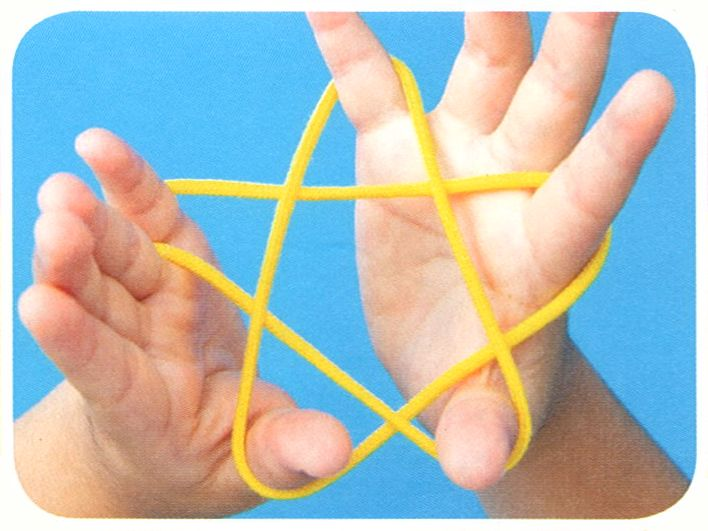
\includegraphics[width=0.3\columnwidth]{figures/figure1.jpg}
\note<.(1)>[item]{these photos comes from this book, translated as "String Figure Encyclopedia" by Noguchi}
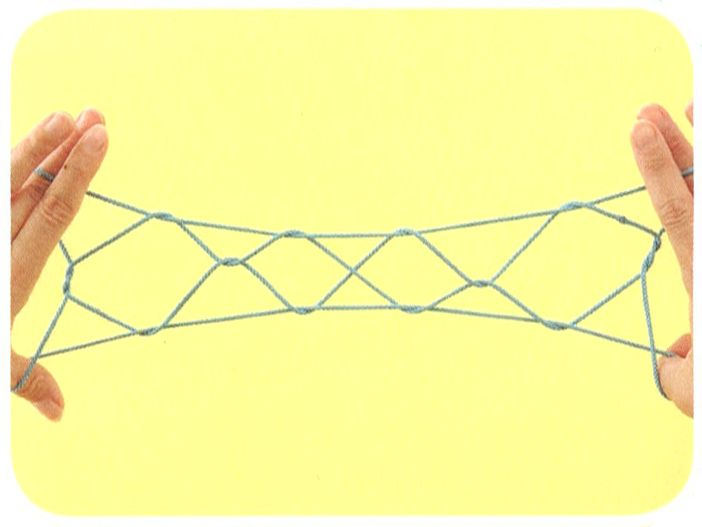
\includegraphics[width=0.3\columnwidth]{figures/figure2.jpg}
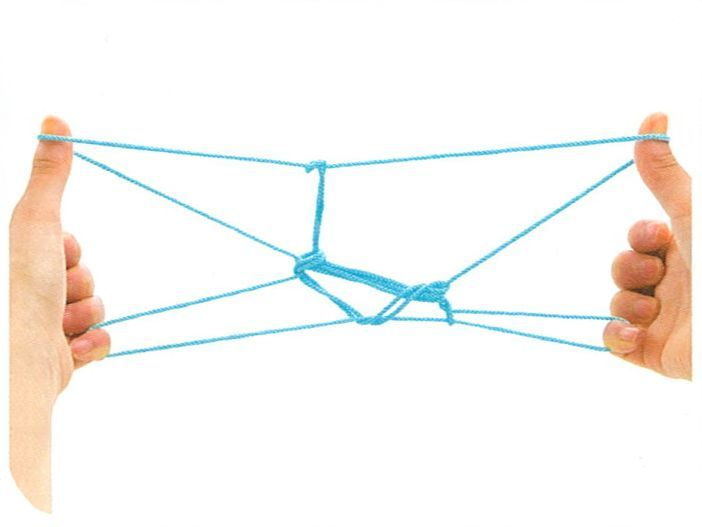
\includegraphics[width=0.3\columnwidth]{figures/figure3.jpg}
\note<.(1)>[item]{i can play the first two, the last one takes like 40 steps to make (CAMERA)}
\end{center}

\begin{itemize}
    \item Designs formed from a loop of string
    \item Commonly known as a children's game
    \note<.(1)>[item]{i mean, look at how young those hands are}
\end{itemize}

People have also been playing with the string throughout history.

\begin{itemize}
    \item  Entertainment during polar nights in the Arctic region
    \note<.(1)>[item]{the native inhabitants in the arctic region play string figures for entertainment }
    \item  Storytelling and illustrating scenes from myths and legends
    \note<.(1)>[item]{the indigenous people in New Zealand play string figures for storytelling and illustrating scenes from myths and legends}
    \note<.(1)>[item]{and i play string figures when overleaf takes forever to compile my slides}
\end{itemize}


\footnote{Noguchi, T. (2020). Ayatori Daizenshu. Shufunotomosha. }

\end{frame}



\begin{frame}{A Computational Approach}

\note<1>[item]{we want to answer the question: how to make string figures}

To make a string figure:

\begin{itemize}
    \item Start with an initial position (opening)
    \note<.(1)>[item]{show opening for star}
    \item Apply a sequence of moves
    \note<.(1)>[item]{make star}
    \item Each move transforms a string figure to another
    \note<.(1)>[item]{show SF after each move}
    \note<.(1)>[item]{...but it has always been a challenge to describe the SFs and these movements to someone else}
    \note<.(1)>[item]{and maybe do some calculations to predict what's the result of applying certain movements}
\end{itemize}

String figures computations

\begin{itemize}
    \item Represent string figures: simple, precise
    \note<.(1)>[item]{it'd be good to have a way that computers understand, so we can store them easily in computers}
    \item Apply moves directly to the representations
    \note<.(1)>[item]{instead of doing the moves physically on a string, then writing the repr down, it'd be good to have an alg to calculate it directly}
    \note<.(1)>[item]{this is essentially teaching computers how to make string figures}
\end{itemize}

Motivation

\begin{itemize}
    \item Precise language of describing string figures
    \note<.(1)>[item]{think of it like music scores}
    \note<.(1)>[item]{if i want to show you how to play this new piece of music}
    \note<.(1)>[item]{i don't have to play it physically with an instrument}
    \note<.(1)>[item]{i can just give you the music sheet}
    \note<.(1)>[item]{which is much more convenient than, say, a recording of me playing the music}
    \note<.(1)>[item]{...}
    \note<.(1)>[item]{music sheet is very visual and hard for computers to read, that's why we have MIDI, and now computers can play MIDI files to simulate what they would sound like on an instrument}
    \item Computer simulations \& animations
    \note<.(1)>[item]{same idea applies with strings figures}
    \note<.(1)>[item]{with a carefully designed language to describe string figures, we can let computers do simulations as well}
    \note<.(1)>[item]{and there are currently implementations of this, made by Alfredo, a physics professor in italy.}
    \note<.(1)>[item]{i can show some features that he implemented at the end of the talk}
    \note<.(1)>[item]{discussing about his code and meeting with parker and another math professor in Université Paris Cité, eric, was part of my reading course for parker}
\end{itemize}

\end{frame}
